%TODO agregar el desfazage de puertos entre modelica y powerdevs.
% agregar una guia con detalles de cada capitulo con los aportes.
%agregar ejemplo jerarquico de un nivel : ejemplo con powerdevs.
%powerdevs implemente los modelos vectorials, más detalles del tamaño
%presentar los bloques vectoriales que se usan

% 
% agregar trabajos futuros
% Agregar size a los modelos powerdevs que transforman conexiones vectores en escalares

\documentclass[a4paper,	11pt]{report}
%-----------Paquetes-------------------------
\usepackage[utf8]{inputenc}
\usepackage{amsmath}
\usepackage[spanish]{babel}
\usepackage{amssymb}
\usepackage{minted}
\usepackage[hidelinks]{hyperref}
\usepackage[lined,boxed,spanish,onelanguage]{algorithm2e} 
\usepackage{graphicx}
\usepackage{booktabs}
%\renewcommand{\abstractname}{Resumen: }

\begin{document}

\renewcommand\floatpagefraction{.9}
\renewcommand\topfraction{.9}
\renewcommand\bottomfraction{.9}
\renewcommand\textfraction{.1}
\setcounter{totalnumber}{50}
\setcounter{topnumber}{50}
\setcounter{bottomnumber}{50}

\title{Conversión de modelos PowerDEVS al lenguaje Modelica}
\author{Tesinista: Luciano Andrade \\ Director: Federico Bergero, Co-Director: Ernesto Kofman} 


\begin{titlepage}
\begin{center}

\huge \bfseries Conversión de modelos PowerDEVS al lenguaje Modelica

\vfill

\begin{minipage}[t]{0.4\textwidth}
\begin{flushleft} \large
\emph{Tesinista :}\\
Luciano Andrade
\end{flushleft}
\end{minipage}\\ 
\vfill
\begin{minipage}[t]{0.4\textwidth}
\begin{flushleft} \large
\emph{Director :}\\
Federico Bergero
\end{flushleft}
\end{minipage}%
\begin{minipage}[t]{0.4\textwidth}
\begin{flushright} \large
\emph{Co-Director:} \\
Ernesto Kofman 
\end{flushright}
\end{minipage}

\vfill


\includegraphics[width=0.25\textwidth]{logo-unr}

\vfill

{\large \today}
\end{center}
\end{titlepage}


\tableofcontents

\begin{abstract}
En este trabajo se describe la implementación de una aplicación para convertir modelos descriptos en la herramienta PowerDEVS\cite{BK11} a modelos en el lenguaje Modelica\cite{Fritzson02modelica--}, más especificamente en $\mu$Modelica\cite{Ber12}, con el fin de aprovechar la velocidad de simulación del 'QSS Solver', permitiendo describir las simulaciones en el entorno PowerDEVS y ejecutando las simulaciones en 'QSS Solver'\cite{Fer12}
\end{abstract}


\chapter{Introducción}

En este trabajo se describe la implementación de una aplicación para convertir modelos descriptos en la herramienta PowerDEVS\cite{BK11} a modelos en el lenguaje Modelica\cite{Fritzson02modelica--}, más especificamente en $\mu$Modelica\cite{Ber12}, en el primer capitulo presentamos las principales motivaciones y objetivos, así como trabajos relacionados y el alcance de este trabajo. En el capitulo dos se recorren conceptos previos, principalmente los formalismo DEVS. En el capitulo tres es donde se muestra en detalles el proceso de conversión de modelos, por ultimo, en el capitulo cuatro, vemos los resultados del trabajo comparando los tiempos de ejecución de los modelos originales y las versiones convertidas a $\mu$-modelica.

\begin{figure}[H]
\centering
 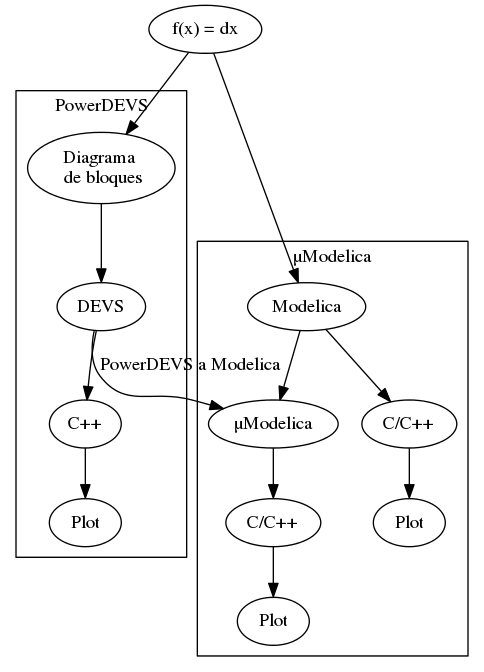
\includegraphics[width=\linewidth]{esquema}
\end{figure}


\section{Motivación y Objetivos}
PowerDEVS\cite{BK11} es una herramienta de simulación de sistemas híbridos, basado en el formalismo DEVS\cite{Zeigler:2000:TMS:580780}, con una interfaz grafica orientada a bloques, donde los bloques pueden ser conectados entre si, modificado los parámetros, además permite conectarse con el entorno Scilab para poder utilizar expresiones y herramientas de cálculo provistas por este entorno.

La resolución de ecuaciones diferenciales ordinarias, requiere el uso de métodos de integración numérica. Todos los algoritmos tradicionales de integración se basan en la discretización de la variable independiente (que generalmente representa el tiempo).

Las rutinas que implementan estos algoritmos, se denominan solvers y existen gran variedad de implementaciones de los mismos en diferentes lenguajes de programación. Los Métodos de Integración Numérica QSS (Quantized State System), a diferencia de los métodos de integración tradicionales, realizan la discretización sobre las variables de estado. En consecuencia, convierten los sistemas continuos en sistemas de eventos discretos, y tienen grandes ventajas para simular sistemas con discontinuidades.

Si bien PowerDEVS, implementa la totalidad de los algoritmos de QSS, resultan ineficientes, dado que malgastan gran parte de la carga computacional en la transmisión de eventos entre submodelos.

Para solventar este hecho se desarrollo una familia de QSS stand-solver, el cual requiere un modelo descripto en lenguaje C el cual contiene las ecuaciones diferenciales, las funciones de cruce de cero asi como la información estructural requerida por los algoritmos QSS. Estos solvers obtienen una mejora de performace de hasta un orden de maginitud comparado con otras implementaciones DEVS.

Sobre este se desarrollo una herramienta la cual genera a partir de un modelo $\mu$-Modedelica \cite{Ber12} (un subconjunto del lenguaje Modelica) el modelo requerido para el QSS solver.

Con el objetivo de utilizar los mejoras de velocidad y mantener un entorno amigable con el usuario, se creo una herramienta capas de convertir un modelo PowerDEVS en un modelo $\mu$-Modelica.


\section{Trabajo relacionado}
En \cite{Ber12} se describe una extensión del Compilador OpenModelica el cual traslada modelos regulares Modelica a $\mu$-modelica. 
ModelicaDEVS \cite{Beltrame06quantisedstate} es una librería Dymola que permite describir simulaciones DEVS en el Modelica, más específicamente en el entorno Dymola.
M/CD++ \cite{conf/mascots/DAbreuW05} es una herramienta para convertir simulaciones en un subconjunto de Modelica, a simulaciones DEVS.
DESlib \cite{Sanz09paralleldevs} es una librería para la descripción de modelos Parallel DEVS en Modelica.


\section{Alcance}
DEVS\cite{Zeigler:2000:TMS:580780}, Discrete Event System Specification (Especificación de Sistemas de Eventos Discretos), es un formalismo modular y jerárquico para modelar y analizar sistemas que pueden ser de eventos de tiempo discreto mediante tablas de transición, y con estados continuos que pueden ser descriptos por ecuaciones diferenciales.
En el formalismo clásico DEVS, los modelos atómicos capturan el comportamiento del sistema, mientras los modelos Acoplados describen la estructura del sistema.
En particular los modelos atómicos en PowerDEVS son descriptos en clases C++, mientras que la estructura se encuentra definida en archivos pds y pdm.
Modelica es un lenguaje de modelado, orientado a objetos, declarativo, para el modelado orientado a componentes de sistemas complejos.
Para poder realizar nuestro objetivo es necesario primero contar con un modelo  en modelica\cite{Fritzson02modelica--} para cada atómico PowerDEVS\cite{BK11} que deseemos convertir. 

De esto se desprenden las siguientes limitaciones importantes:
\begin{itemize}
	\item La semántica de los modelos convertidos depende de los modelos equivalentes a los DEVS atómicos 
	\item Solamente podemos convertir modelos cuyos componentes atómicos estén o puedan ser convertidos a $\mu$modelica.
\end{itemize}

	
\chapter{Conceptos Previos}
En este capítulo introducimos algunos conceptos básicos, necesarios para poder comprender este trabajo, modelado y los formalismos y simulación de sistemas y clasificación.

\section{Modelado y Simulación}
Modelado y Simulación de un Sistema es el proceso por el cual se desarrolla un modelo, el cual es luego simulado, de forma de obtener datos sobre el sistema. El modelo debe conservar las principales características del sistema, pero al mismo tiempo ser significativamente más simple, de forma que al momento de simularlo sea más eficaz utilizar la simulación que el sistema en si.

\subsection{Sistemas Continuos y Discretos}
Se considera un sistema continuo si las variables de este son conocidas en cada instante de tiempo, mientras que se considera discreto si las variables son conocidas en instantes de tiempo determinados.

En general los sistemas en estudio serán continuos, pero deberemos utilizar sistemas discretos puesto que la simulación en computadora así lo requiere, puesto que la misma computadora es un sistema discreto.

\subsection{Métodos de Integración numérica}
Un sistema continuo puede ser descripto por un modelo en espacios de estados de la forma:

\begin{equation} \label{eq1}
x(t) = f (x(t), u(t))
\end{equation}

donde $x \in \Re^n$  es el vector de estados, $u \in \Re^m$ es una función de entradas conocidas,
$t$ representa el tiempo y con sus condiciones iniciales:

\begin{equation} \label{eq2}
x(t = t_0 ) = x_0
\end{equation}

Sea $x_i (t)$ la trayectoria del estado $i$-esimo expresada como función de tiempo simulado. 
Mientras que la ecuación \eqref{ eq1 } no contenga discontinuidades $x_i (t)$ será una función continua con derivada continua. Esta puede ser aproximada con la precisión deseada mediante series de Taylor en cualquier punto de su trayectoria

Denominando $t^{\ast}$ al instante de tiempo en torno al cual se aproxima la trayectoria mediante una serie de Taylor, y siendo $t^{\ast} + h$ el instante de tiempo en el cual se quiere evaluar la aproximación, entonces, la trayectoria en dicho punto puede expresarse como sigue:

\begin{equation} \label{eq3}
x_i(t^* + h) = x_i(t^*) + \frac{dx_i (t^*)}{dt} \cdot h + \frac{d^{2}x_i (t^*)}{dt^2} \cdot \frac{h^2}{2!} + \cdots
\end{equation}

Reemplazando con la ecuación de estado \eqref{eq1}, la serie \eqref{eq3} queda:

\begin{equation} \label{eq4}
x_i(t^* + h) = x_i(t^*) + f_i(t^*) \cdot h + \frac{d^{2}x_i (t^*)}{dt^2} \cdot \frac{h^2}{2!} + \cdots
\end{equation}

Los distintos algoritmos de integración difieren en la manera de aproximar las derivadas superiores de $f$ y en el número de términos de la serie de Taylor que consideran para la aproximación.

\section{Formalismo DEVS}
DEVS es un formalismo para modelar y analizar sistemas de eventos discretos (es decir, sistemas en los cuales en un lapso finito de tiempo, ocurren una cantidad finita de eventos).
Un modelo DEVS puede ser visto como un autómata que procesa una serie de eventos de entrada y genera una serie de eventos de salida. Este procesamiento está regido por la estructura interna de cada una de las partes que componen el modelo general.
Un modelo DEVS está descripto por dos clases de componentes, modelos atómicos y modelos acoplados.

\subsection{Atómicos}
Un modelo atómico representa la unidad "indivisible" de especificación, en el sentido que es la pieza fundamental y más básica de un modelo DEVS. Formalmente un modelo atómico está conformado por la 7-upla:

\begin{equation} 
(X, Y, S, \delta_{int} , \delta_{ext}, \lambda, t_{a}) \mbox{ donde :}
\end{equation}

\begin{itemize}
\item $X$ es el conjunto de valores de entrada que acepta el modelo atómico, es decir un evento de entrada tiene como valor un elemento del conjunto X.
\item $Y$ es el conjunto de valores de los eventos de salida que puede emitir el modelo atómico.
\item $S$ es el conjunto de estados internos del modelo, en todo momento el atómico está en un estado dado, que es un elemento del conjunto S.
\item $ta$ es una función $S \to R^{+}$ , que indica cuánto tiempo el modelo atómico permanecerá en un estado dado, si es que no se recibe ningún evento de entrada. Esta función puede asociarse también al tiempo de vida de un estado.
\item $\delta_{int}$ es una función $S \to S$, que indica la dinámica del sistema en el momento que el modelo atómico realiza una transición interna. Sería el análogo a una tabla de transición en otros autómatas.
\item $\delta_{ext}$ es una función $(S \times R^{+} \times X) \to S$, que indica el cambio de estado ante la presencia de un evento externo.
\item $\lambda$ es una función $S \to Y$ que indica qué evento se debe emitir al salir de un estado dado.
\end{itemize}

Los conjuntos $S$, $X$ e $Y$ son arbitrarios, y en general infinitos. Cada posible estado $s$ ($s \in S$) tiene asociado un Avance de Tiempo calculado por la Función de Avance de Tiempo $ta(s)$.
En la Figura \ref{fig:fig2-5} vemos la evolución de un modelo atómico. Si el estado toma el valor $s_1$ en el tiempo $t_1$ , tras $ta(s_1)$ unidades de tiempo (o sea, en tiempo $ta(s_1 ) + t_1 )$ el sistema realizará una transición interna yendo a un nuevo estado $s_2$ dado por $s_2 = \delta_{int} (s_1 )$. La función $\delta_{int}$ se llama Función de Transición Interna.

Cuando el estado va de $s_1$ a $s_2$ se produce también un evento de salida con valor $y_1 = \lambda(s_1)$. La función $\lambda (\lambda : S \to Y )$ se llama Función de Salida. Así, las funciones $ta$, $\delta_{int}$ y $\lambda$ definen el comportamiento autónomo de un modelo DEVS.

Cuando llega un evento de entrada, el estado cambia instantáneamente. El nuevo valor del estado no sólo depende del valor del evento de entrada sino también del valor anterior del estado y del tiempo transcurrido desde la última transición.

Si el sistema llega al estado $s_3$ en el instante $t_3$ y luego llega un evento de entrada en el instante $t_3 + e$ con un valor $x_1$ , el nuevo estado se calcula como $s_4 = \delta_{ext} (s_3 , e, x_1 )$ (notar que $ta(s_3 ) > e$). En este caso se dice que el sistema realiza una transición externa. La función $\delta_{ext}$ se llama Función de Transición Externa. Durante una transición externa no se produce ningún evento de salida.
\begin{figure}[!htbp]
  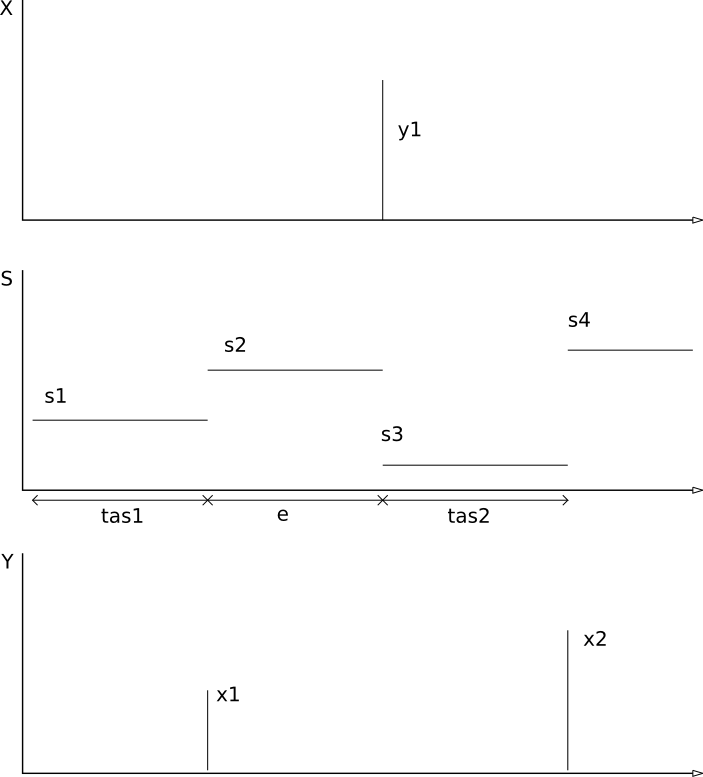
\includegraphics[scale=0.5]{devs-atomic}
  \caption{Comportamiento de un modelo DEVS atómico}
   \label{fig:fig2-5}
\end{figure}

\subsection{Acoplados}
La descripción de un sistema puede ser completamente realizada utilizando modelos atómicos, aunque esto resulta un poco incómodo y confuso. Los conjuntos de estados y las funciones de transición se vuelven inmanejables en sistemas complejos, y nunca podemos asegurar haber cubierto todos los posibles estados.
Para abordar este problema, el formalismo DEVS introduce lo que se llaman modelos acoplados, que es una forma de agrupar modelos DEVS y generar nuevos modelos a partir de este agrupamiento.
Hay dos formas de acoplamiento, la más general, en la cual se utilizan funciones de traducción entre los sub–sistemas y otra clase que adopta el uso de puertos para la comunicación entre sub–sistemas. Aunque estas dos formas son equivalentes entre sí, describiremos la segunda clase, ya que es la más simple y es la utilizada en el presente trabajo.
Formalmente un modelo acoplado está representado por la octo-upla:

\begin{equation}
N = (X_N , Y_N , D, {M_d }, EIC, EOC, IC, Select)
\end{equation}

donde cada componente es:
\begin{itemize}
\item $X_N$ es el conjunto de eventos de entrada al modelo acoplado, representado por el producto cartesiano del conjunto de puertos de entrada $InPorts$ y el conjunto de posibles valores para cada puerto. O sea un evento de entrada al modelo acoplado está representado por un par $(p, v)$ donde $p \in InPorts$ y $v \in X_p$ .

\item $Y_N$ es el conjunto de eventos que el modelo puede emitir. Es un elemento del producto cartesiano entre el conjunto de puertos de salida $OutPorts$ y el conjunto de posibles valores para este puerto, o sea un evento de salida del modelo acoplado está representado por un par $(p, v)$ donde $p \in OutPorts$ y $v \in Y_p$.

\item $D$ es el conjunto de los índices a los modelos DEVS (atómicos y acoplados) que conforman este modelo. 

\item ${M_d}$ es el conjunto de los modelos atómicos y/o acoplados (son justamente los modelos que "acopla" o "agrupa" este modelo acoplado).

\item EIC y EOC son el conjuntos de conexiones entre los modelos internos y los puertos del modelo acoplado:
      \begin {itemize}
          \item EIC (o External Input Coupling) son las conexiones de entrada al acoplado, es decir, conecta un puerto de entrada del acoplado con un puerto de entrada de un modelo perteneciente al acoplado.
          \item EOC (o External Output Coupling) son las conexiones de salida del acoplado. Conecta un puerto de salida de un modelo interno del acoplado con un puerto de salida del acoplado. Formalmente:
          $ EIC \in \{((N, ip_N ), (d, ip_d )) | ip_N \in InPorts, d \in D, ip d \in InPorts_d \} $
          $EOC \in \{((d, op_d ), (N, op_N ))  | op_N \in OutPorts, d \in D, op d \in OutPorts_d \} $
    
    	donde N es el modelo acoplado.
      \end{itemize}

\item $IC$ representa las conexiones internas del modelo acoplado donde:
\begin{equation}
IC \in \{((a, ip_a ), (b, ip_b )) | a, b \in D, ip a \in OutPorts_a , ip_b \in InPorts_b \}
\end{equation}
donde no se permite que $a = b$.

\item Select es una función $(D \times D \to D)$ que decide qué modelo realizará primero su transición interna, si se da el caso de eventos simultáneos. Es una función de "desempate" que en ciertos modelos es necesaria.
\end{itemize}

$InPorts$ y $Outports$ son conjuntos que describen los posibles puertos de entrada y salida respectivamente. En general se utilizan números enteros para representar los puertos posibles por lo cual $InPorts = \mathbb{N}$ y $Outports = \mathbb{N}$ Los modelos acoplados son en sí mismos modelos DEVS válidos; formalmente el acoplamiento (como lo definimos antes) es una operación cerrada sobre el conjunto de modelos DEVS. Acoplar modelos DEVS forma nuevos modelos DEVS. Sin esta cualidad el acoplamiento resultaría inútil desde del punto de vista del formalismo. También trae muchas ventajas a la hora de describir modelos DEVS y a la hora de simularlos. El acoplamiento da lugar a una estructura jerárquica de desarrollo.

En esta Sección introducimos una extensión al formalismo DEVS para especificar modelos vectoriales fácilmente.

\subsection{Modelos DEVS parametrizados}
Definimos aquí primero un modelo DEVS parametrizado. Dado un modelo DEVS atómico $M$ obtenemos un Modelo DEVS Parametrizado:
\begin{equation}
M (p) = \{X, Y, S, \delta_{int} p , \delta_{ext} p ,\lambda p , ta p\}
\end{equation}

donde $p \in P$ es un parámetro que pertenece a un conjunto de parámetros arbitrario tal que $\delta_{int}$ , $\delta_{ext}$ , $\lambda$ y $ta$ dependen también de $p$.
Notar que dos modelos DEVS $M (p_1 )$, $M (p_2 )$ con $p_1 \neq p_2$ pueden exhibir distintos comportamientos aunque compartan los mismos conjuntos de entrada, salida y de estados ($X$, $Y$ , y $S$, respectivamente).

\subsection{Modelos Vectoriales}
Dado el modelo escalar DEVS Parametrizado:
\begin{equation}
M (p) = \{X, Y, S, \lambda_{int} , \lambda_{ext} , \lambda, ta, p\}
\end{equation}

definimos un modelo Vectorial DEVS como la estructura:
\begin{equation}
V D = \{N, XV, Y V, P, {M i }\},
\end{equation}
donde:
\begin{itemize}
\item $N \in N$ es la dimensión del modelo vectorial.

\item $XV = X \times Index$ es el conjunto de eventos de entradas vectorial donde $X$ es el conjunto de eventos de entrada del modelo escalar e $Index = {1, \ldots , N }$ es el conjunto de índices que indican cuál de los modelos DEVS atómicos recibirá el evento.

\item $YV = Y \times Index$ es el conjunto de eventos de salida vectorial donde $Y$ es el conjunto de eventos de salida del modelo escalar e $Index = {1, \ldots , N }$ es el conjunto de índices que indica que modelo escalar de los $N$ , emitió el evento. %TODO : check Index = 0...N?

\item $P$ es un conjunto de parámetros arbitrario.

\item Para cada índice $i \in Index$, $p(i) \in P$ es un parámetro y $M_i = M (p(i))$ es el modelo DEVS Parametrizado escalar.
\end{itemize}
	
\section{Métodos de integración QSS}
Quantized State System methods (métodos de QSS), pueden aproximar Ecuaciones Diferenciales Ordinarias (ODE por sus siglas en inglés) mediante modelos de eventos discretos. Formalmente, el método de QSS de primer orden (llamado QSS1) aproxima la ecuación por:

\begin{equation}
\dot{x}(t) = f (q(t), v(t))
\end{equation}

donde $q$ es el vector de estados cuantificados y sus componentes están relacionadas una a una con las del vector de estados $x$ siguiendo una función de cuantificación con histéresis:

\begin{equation}
q_j(t) = \left\{ 
  \begin{array}{l l}
    x_j(t)  \quad \text{si} \mid x_j (t ) - q_j (t^{-} ) \mid \geq \Delta Q_j \\
    q_j (t^{-} ) \quad \text{en caso contrario}
  \end{array} \right.
\end{equation}

donde $q_j (t^{-})$ es el límite por izquierda de $q_j$ en $t$.

\begin{figure}[!htbp]
  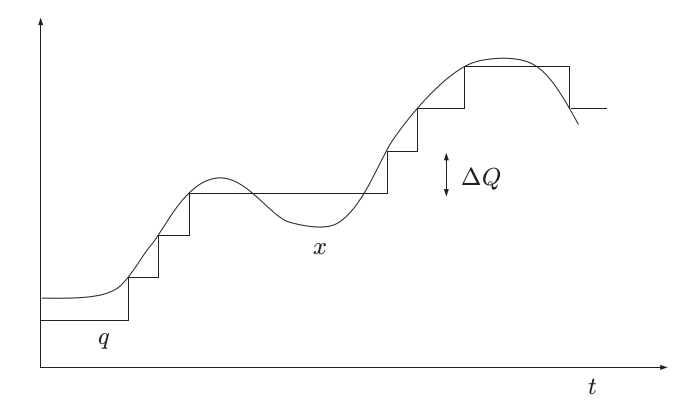
\includegraphics[scale=0.5]{histeresis1}
  \caption{Comportamiento de un modelo DEVS atómico}
   \label{fig:fig2-2}
\end{figure}

En la Figura \ref{fig:fig2-2} vemos la relación entrada-salida de una función de cuantificación de orden cero.

Notar que un cuantificador con histéresis tiene memoria. Es decir, calcula $q(t)$ no sólo en función del valor actual de $x(t)$ sino también de su valor pasado.
La presencia de esta función que relaciona $q_j (t)$ y $x_j (t)$ implica que $q_j (t)$ sigue una trayectoria constante a trozos que sólo cambia cuando difiere con $x_j (t)$ en un parámetro $\Delta Q_j$ llamado quantum.

Las variables $q_j$ son llamadas variables cuantificadas y pueden ser vistas como una aproximación constante a trozos de la variable de estado correspondiente $x_j$. De la misma forma las componentes de $v(t)$ son aproximaciones constantes a trozos de las componentes correspondientes de $u(t)$.  Los pasos de integración en los métodos de QSS sólo se producen cuando una variable cuantificada $q_j (t)$ cambia, esto es, cuando la variable de estado correspondiente $x_j (t)$ difiere de $q_j(t^{-})$ en un quantum. Ese cambio implica también que algunas derivadas de estado (aquellas que dependen de $x_j$ ) también son modificadas. Luego, cada paso involucra un cambio en sólo una variable cuantificada y en algunas derivadas de estado. Por lo tanto cuando un gran sistema ralo (o sparse) posee sólo actividad en unos pocos estados mientras que el resto del sistema se mantiene intacto, los métodos de QSS explotan intrínsecamente este hecho realizando cálculos sólo donde y cuando ocurren los cambios.
Otra ventaja importante de los métodos de QSS es que tratan las discontinuidades de una manera muy eficiente. Dependiendo del orden del método, las variables de estado siguen trayectorias lineal a trozos, parabólica a trozos o constante a trozos. Debido a ello, detectar los cruces por cero es sencillo ya que se debe resolver una ecuación cúbica en el peor caso. Una vez que la discontinuidad es detectada, el algoritmo la trata como un paso normal ya que cada paso es de hecho una discontinuidad en una variable cuantificada. Por lo tanto la ocurrencia de una discontinuidad implica sólo algunos cálculos locales para re-computar las derivadas de estados que están directamente afectadas por ese evento.
Estas ventajas resultan en una aceleración notable en el tiempo de simulación contra los algoritmos de integración numérica clásicos. En modelos con discontinuidades frecuentes como sistemas de electrónica de potencia, los métodos de alto orden que veremos a continuación, pueden simular hasta 20 veces más rápido que los métodos convencionales.

\section{PowerDEVS}
PowerDEVS es un programa, concebido para ser utilizado por expertos programadores DEVS, así como usuarios finales que solo quieren conectar bloques y simular.

PowerDEVS esta compuesto por varios programas independientes:
\begin{itemize}
\item El \emph{editor de modelos}, es desde el punto de vista del usuario, el principal programa de PowerDEVS, pues provee la interfaz gráfica y enlaces para las demás aplicaciones. 
Además de construir, manejar modelos y librerías, permite lanzar las simulaciones (lanzando el \emph{Pre procesador}) y editar los bloques elementales hasta su definición atómica de modelo (invocando el \emph{Editor Atómico}).
La ventana principal de \emph{Editor de Modelo} permite al usuario crear y abrir modelos y librerías. También permite a las librerías ser exploradas y los bloques arrastrados de las librerías a los modelos.
También existen algunas características avanzadas que pueden ser manejadas desde la ventana principal como establecer cual es la librería activa, y configurar las barras de herramientas y menúes para invocar aplicaciones externas.
La ventana del Modelo provee todas las funcionalidades típicas para la edición gráfica para poder copiar, cambiar el tamaño, rotar, etc. mientras que las conexiones pueden ser dibujadas entre los diferentes puertos.
La ventana de Edición de Bloques, nos permite configurar la apariencia gráfica y elegir los parámetros del bloque y, en el caso de los modelos atómicos, seleccionar el archivo que contiene el código asociado con la definición DEVS.

\item El \emph{Editor de Atómico} facilita la edición del código C++ correspondiente a cada modelo atómico DEVS, el usuario solo debe definir las variables que forman el estado y la salida del modelo DEVS. Luego, el código C++ de la transición de avance de tiempo y la función de salida deben se completados. Hay dos ventanas adicionales init y exit, donde se puede completar con código que sera ejecutado al inicio y fin de la simulación.
Cuando el modelo se guarda, el código es guardado en los archivos .cpp y .h. 

\item El \emph{Pre procesador}, toma un archivo .pdm (o .pds) producido por el \emph{Editor de Modelos} y produce el programa que corre la simulación. Básicamente traduce el archivo .pdm a un archivo de cabecera .h que enlaza el simulador y el coordinador de acuerdo a la estructura del modelo pasando además los parámetros definidos para el modelo.
El \emph{Pre procesador}, además produce un makefile (Makefile.include) el cual invoca el compilador para generar el programa que implementa la simulación. 

\item La \emph{interfaz de simulación}, que corre el programa que implementa la simulación y permite variar parámetros de la simulación como tiempo final, números de simulación a ejecutar, y el modo de simulación (normal, cronometrada, pasa o paso, etc.).

\item Una instancia de Scilab, que actua como un espacio de trabajo, donde los parámetros pueden ser leídos, y los resultados pueden ser exportados. 
\end{itemize}

\section{Modelica}
Modelica es un lenguaje de alto nivel, orientado a objetos para el modelado de grandes, complejos y sistemas heterogéneos.
Modelos en Modelica son descriptos matemáticamente por ecuaciones diferenciales, algebraicas y discretas. Sub-modelos pueden ser interconectados para crear modelos más complejos y hay varias herramientas para combinar modelos en forma gráfica. 
Hay varios compiladores para convertir modelos de Modelica en código de simulación. Entre las más populares podemos mencionar Dymola y OpenModelica

\section{Stand–Alone QSS solver}
Como mencionamos antes los métodos QSS de integración remplazan la discretización del tiempo de los métodos clásicos por una quantificación de las variables del sistema. De esta forma, estos métodos generan aproximaciones del sistema continuo y tienen algunas ventajas sobre sus contra partes clásicas.

La forma más simple de implementar algoritmos QSS es mediante el uso de un simulador DEVS. Estas implementaciones aunque simples, son ineficientes, pues desperdician mucho poder computacional en sincronizar y transmisión de eventos.

Estas desventajas motivo el desarrollo del \emph{Stand–Alone QSS solver}, implementados como un conjunto de módulos en lenguaje C. Este implementa toda la familia de métodos QSS y permite que los modelos contengan discontinuidades de tiempo y estado.

Una dificultad impuesta por los métodos QSS es que hace uso de información estructural del modelo. Cada paso en un método QSS involucra un cambio en una variable de estado y en la derivada del estado que depende de el. Por lo que el modelo debe proveer no solo la expresión para calcular las derivadas del estado (como en un clásico ODE solver) pero además un matriz de incidencias para informar al solver que derivadas de estado han cambiado luego de cada paso.

Como sería muy incomodo para el usuario proveer esta información estructural, el solver tiene una interfaz que automáticamente obtiene la matriz de incidencia desde una definición estándar de modelos.

La interfaz permite al usuario describir el modelo utilizando un subconjunto del lenguaje estándar de Modelica ($\mu$Modelica) y automáticamente genera el código C del modelo incluyendo la estructura.

\subsection{$\mu$Modelica}
El lenguaje $\mu$Modelica tiene las siguientes restricciones con respecto a Modelica:

\begin{itemize}
 \item El modelo es plano, es decir no permite clases.
 \item Todas las variables pertenecen al tipo predefinido Real y solo hay tres categorías de variables: estado continuo, estado discreto y variables algebraicas.
 \item Los parámetros también son de tipo Real. 
 \item Arreglos están permitidos. Indices en los arreglos dentro de clausulas for están restringidos a la forma $\alpha \cdot i + \beta$, donde $\alpha$ y $\beta$ son expresiones enteras y $i$ es el indicie de la iteración.
 \item La sección de ecuaciones esta compuesta de :
 \begin{itemize}
	\item Definición de variables de estados : $der(x) =  f (x(t), d, a(t), t);$ ODE en forma explicita
	\item Definición algebraica : $(a_1 , \dots , a_n ) = g(x(t), d, a(t), t);$
 \end{itemize}
 con la restricción de que cada variable algebraica solo puede depender del estado y de variables algebraicas previamente definidas.
 
 \item Discontinuidades son expresadas solo con las clausulas $when$ y $elsewhen$ dentro de la sección $algorithm$. Las condiciones dentro de las dos clausulas solo pueden ser relaciones ($<$, $\leqslant$, $>$ $\geqslant$) y, dentro de la clausula, solo asignaciones de variables discretas y $reinit$ de estados continuos son permitidos
\end{itemize}


\chapter{Conversión de modelos DEVS}

En este capitulo se describe la conversión de los modelos DEVS a modelos Modelica.

\section{Modelos Atómicos}

Los modelos atómicos no son traducidos automáticamente, deben ser provistos siguiendo la siguiente especificación:

\begin{itemize}
\item El código debe ser Modelica ($\mu$modelica) valido y estar ubicado en el mismo directorio del código C que el modelo atómico PowerDEVS, con el mismo nombre que el archivo .h, pero con extensión .mo
\item Los parámetros del modelo DEVS deben ser pasado en el parámetro $p$
\item Los valores de entrada del modelo son asociados a la variable $u$
\item Los valores de salida del modelos son asociados a la variable $y$
% \item La cantidad de ecuaciones y variables debe ser igual.
\end{itemize}

Por ejemplo el código del integrador, originalmente ubicado en el archivo qss\_integrator.h de PowerDEVS, se ubica en el archivo qss\_integrator.mo ambos dentro del directorio qss.

\begin{minted}{modelica}
class QSSIntegrator
  parameter Real p[4]={0,0,0,0};
  parameter Real x0 = p[4];
  Real u[1];
  Real y[1](start = {x0});
equation
  der(y[1]) = u[1];
end QSSIntegrator;
\end{minted}

Los parámetros son remplazadas en el modelo, evaluados en Scilab, lo que los transforma en float, los cuales son presentados como reales (Real) en el código.

Los modelos no encontrados son ignorados en la traducción.

\section{Modelos Acoplados Planos}

Llamamos \emph{Modelos Acoplados Planos} a los Modelos Acoplados que solo contienen \emph{Modelos Atómicos}. Estos modelos son convertidos en modelos Modelica de la siguiente forma:
Para el $i$-esimo modelo atómico del modelo acoplado
\begin{itemize}
	\item Se incluye el código Modelica del $i$-esimo modelo atómico
	\item Se remplazan los parámetros $p$ por los del $i$-esimo modelo atómico.
	\item Se reescriben todas las variables (excepto la variable $time$) construido con $i$ y el nombre del modelo (en Modelica).
\end{itemize}

Luego cada conexión entre Modelos Atómicos es replicada en el código de Modelica resultante. Los modelos Atómicos cuyo entrada (o salida) son escalares son conectados con un ecuación del tipo $u = y$ mientras que los modelos vectoriales son conectados con la misma ecuación, solo que dentro de un $for$.

Veamos como se realiza la transformación paso a paso con un ejemplo de un integrador.

\begin{figure}[!htbp]
\begin{center}
  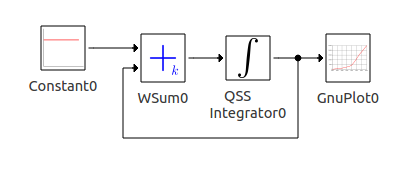
\includegraphics[scale=0.5]{integrator-devs}
  \caption{DEVS Ejemplo de Integrador}
  \end{center}
   \label{fig:integrator}
\end{figure}

Este modelo incluye los siguientes modelos atómicos:
\begin{itemize}
	\item Constante: Constant0
\begin{minted}{modelica}	
class Constant
  parameter Real k = 1;
  Real y[1];
equation
  y[1] = k;
end Constant;	
\end{minted}

	\item Sumador: WSum0
\begin{minted}{modelica}	
class WSum
  parameter Real p[9]={0,0,0,0,0,0,0,0};
  parameter Integer n= integer(p[9]);
  parameter Real w[n] = p[1:n];
  Real u[n];
  Real y[1];
equation
  y[1]=u*w;
end WSum;
\end{minted}

	\item Integrador: QSSIntegrator0
\begin{minted}{modelica}	
class QSSIntegrator
  parameter Real p[4]={0,0,0,0,0,0,0,0};
  parameter Real x0 = p[4];
  Real u[1];
  Real y[1](start = {x0});
equation
  der(y[1]) = u[1];
end QSSIntegrator;
\end{minted}

	\item Gnu Plot : GNUPlot0, el cual no va a ser convertido debido a que no tiene un modelo equivalente en modelica.
\end{itemize}

El integrador es el primero en la lista de atómicos dentro del PowerDEVS, por lo que es el primero en procesarse y por lo tanto obtiene el prefijo $<nombre modelo>\_0\_$ para sus variables, también remplazamos los parámetros provenientes de la simulación de PowerDEVS:

\begin{minted}{modelica}	
class QSSIntegrator
  parameter Real QSSIntegrator_0_p[4]={0,1e-06,0.001,0};
  parameter Real QSSIntegrator_0_x0 = 0;
  Real QSSIntegrator_0_u[1];
  Real QSSIntegrator_0_y[1](start = {QSSIntegrator_0_x0});
equation
  der(y[1]) = QSSIntegrator_0_u[1];
end QSSIntegrator;
\end{minted}

\begin{minted}{modelica}
class WSum
  parameter Real WSum_1_p[9]={1,(-1),0,0,0,0,0,0,2};
  parameter Integer WSum_1_n= integer(2);
  parameter Real WSum_1_w[WSum_1_n] = p[1:WSum_1_n];
  Real WSum_1_u[WSum_1_n];
  Real WSum_1_y[1];
equation
  WSum_1_y[1]=WSum_1_u*WSum_1_w;
end WSum;
\end{minted}

\begin{minted}{modelica}	
class Constant
  parameter Real Constant_2_k = 1;
  Real Constant_2_y[1];
equation
  Constant_2_y[1] = Constant_2_k;
end Constant;	
\end{minted}

En este punto podemos juntar las declaraciones y ecuaciones dentro de un nuevo modelo, el cual llamaremos con el nombre del modelo a convertir.

\begin{minted}{modelica}	
class Integrador
  parameter Real QSSIntegrator_0_p[4]={0,1e-06,0.001,0};
  parameter Real QSSIntegrator_0_x0 = 0;
  Real QSSIntegrator_0_u[1];
  Real QSSIntegrator_0_y[1](start = {QSSIntegrator_0_x0});
  parameter Real WSum_1_p[9]={1,(-1),0,0,0,0,0,0,2};
  parameter Integer WSum_1_n= integer(2);
  parameter Real WSum_1_w[WSum_1_n] = p[1:WSum_1_n];
  Real WSum_1_u[WSum_1_n];
  Real WSum_1_y[1];
equation
  der(y[1]) = QSSIntegrator_0_u[1];
  WSum_1_y[1]=WSum_1_u*WSum_1_w;
  Constant_2_y[1] = Constant_2_k;
end QSSIntegrator;
\end{minted}

Luego de agregar las equaciones correspondientes a las interconecciones de los modelos atómicos, obtenemos el siguiente modelo
	
\begin{minted}{modelica}
model Integrador
  parameter Real QSSIntegrator_0_p[4] = {0,1e-06,0.001,0};
  parameter Real QSSIntegrator_0_x0 = 0;
  Real QSSIntegrator_0_u[1];
  Real QSSIntegrator_0_y[1](start = {0});
  parameter Real WSum_1_p[9] = {1,(-1),0,0,0,0,0,0,2};
  parameter Integer WSum_1_n = integer(2);
  parameter Real WSum_1_w[WSum_1_n] = WSum_1_p[1:WSum_1_n];
  Real WSum_1_u[WSum_1_n];
  Real WSum_1_y[1];
  parameter Real Constant_2_k = 1;
  Real Constant_2_y[1];
  equation
    der(QSSIntegrator_0_y[1]) = QSSIntegrator_0_u[1];
    WSum_1_y[1] = WSum_1_u*WSum_1_w;
    Constant_2_y[1] = 1;
    QSSIntegrator_0_u[1] = WSum_1_y[1];
    WSum_1_u[2] = QSSIntegrator_0_y[1];
    WSum_1_u[1] = Constant_2_y[1];
end Integrador;
\end{minted}

\section{Modelos Acoplados Jerárquicos}
%TODO : Demostración por inducción.
%TODO : ¿Que sea cerrado sobre acoplado es lo mismo que sea equivalente?

En la sección anterior mostramos como son convertidos modelos acoplados compuestos por modelos atómicos, para convertir un modelo acoplado jerárquico, es decir con más modelos acoplados internos, vamos a generar un modelo acoplado plano, equivalente al modelo jerárquico inicial.

Para realizar el aplanado, se recorre recursivamente los modelos acoplados

\begin{itemize}
\item por cada modelo acoplado si solo tiene modelos atómicos, es remplazado por los modelos atómicos internos, los cuales se encuentran conectados sin modificaciones excepto por las conexiones externas, las cuales son reasignadas de forma de mantener las conexiones.
\item si el modelo acoplado contiene otros modelos acoplados entonces aplanamos ese modelo recursivamente.
\end{itemize} 

De esta forma obtenemos un modelo con solo modelos atómicos el cual podemos convertir con el procedimiento anterior.

\section{Modelos Vectoriales}
Los modelos vectoriales difieren levemente de los atómicos no vectoriales. Estos modelos pueden tener tanto la entrada como la salida de sus conectores de forma vectorial, por lo que los modelos vectoriales deben indicarlos con la anotación de Modelica $PD2MO$, por ejemplo:
\begin{itemize}
\item $annotation(PD2MO = {Scalar, Vector});$ cuando la entrada es escalar, es decir no vectorial y la salida vectorial
\item $annotation(PD2MO = {Vector, Scalar});$ cuando la entrada es vectorial y la salida vectorial
\item $annotation(PD2MO = {Vector, Vector});$ cuando ambos, la entrada y salida son vectoriales.
\item $annotation(PD2MO = {Scalar, Scalar});$ cuando ambas entrada y salida son escalares, este es el caso por omisión y no es necesario declararlo.
\end{itemize}

Además las variables de entradas $u$ y salidas $y$ vectoriales deben ser definidas como vectores en Modelica. A modo de ejemplo se muestra a continuación el archivo vector/qss\_integrator\_vec.mo. Este modelo atómico representa $N$ integradors y es la version vectorial del integrador atómico mostrado antes.


\begin{minted}{modelica}
class VecInt
  parameter Real p[5] = {0, 10, 0, 0, 10};
  constant Integer N = p[5];
  parameter Real x0 = p[4];
  Real u[N, 1];
  Real y[N, 1];
initial algorithm
  for i in 1:N loop
    y[i, 1] := x0;
  end for;
equation
  for i in 1:N loop
    der(y[i, 1]) = u[i, 1];
  end for;
  annotation(PD2MO = {Vector, Vector});
end VecInt;
\end{minted}


\chapter{Resultados}

\section{Equivalencia semántica de la conversión}
Hay tres situaciones que debemos considera al momento de verificar la equivalencia semántica
\begin{itemize}
\item Modelos Atómicos : Los modelos atómicos son convertidos por el usuario, los que se han propuesto en el código mantienen una conservación de la semántica que no es estricta y se trató manualmente. 
\item Modelos Acoplado - Plano : Como fue descripto en la sección Modelos Acoplados Planos, los modelos son conectados por una ecuación en caso de ser un modelo escalar, o por un conjunto de ecuaciones (expresadas en una sentencia $for$). En este caso esta conversión (conexión por igualdad) solo mantiene una semántica relativa, pues la semántica de una conexión (o grupo de conexiones en el caso vectorial) es diferente de la semántica de un ecuación (o grupos de ecuaciones).

\item Modelo Jerárquico : En este caso si podemos probar la equivalencia semántica, entre el modelo original, es decir un modelo acoplado que incluye más modelos acoplados, con un modelo "aplanado" (solo con modelos atómicos). Esto se debe a que el formalismo DEVS es cerrado bajo el acoplamiento \cite{Zeigler:2000:TMS:580780} y \cite{zeigler1984multifacetted}, lo que permite remplazar un modelos acoplado por equivalentes atómicos, conectados apropiadamente. %TODO : Verificar.
\end{itemize}

\section{Comparación de performance}

%\chapter{Detalles de Implementación}
%API Powerdevs, AST Modelica, programa principal

%modelCoupled *cm = parsePDS(QString::fromStdString(src_infile));
%modelCoupled *qm = flatter::flat(cm);
%generateCode(qm, QString::fromStdString(flatted), false, true);
%
%ofstream oFlogfile;
%oFlogfile.open(logfile.c_str(), ios::trunc);
%
%Pd2Mo q = Pd2Mo();
%q.setPath(path);     
%
% q.transform(flatted, modelname, &outfile, &oFlogfile);
%
%mda *m = new mda();
%prodint *  prod = new prodint();
%If *i = new If();
%outfile.open(mmodelica_src_outfile.c_str(), ios::trunc);
%outfile << m->visitClass( prod->visitClass( i->visitClass( *sd->models()->begin()))) << endl;


\section{Ejemplos de Aplicación}
En esta Sección presentamos dos ejemplos motivadores para la implementación de la conversión, el primer un modelo de una línea de transmisión LC (circuito resonante compuesto por una bobina y un capacitor) utilizando el Método de Líneas DEVS para grandes sistemas \cite{Cel06}, el cual resulta en $N$ segmentos cada uno representado con Vectorial DEVS. Luego analizaremos un ejemplo de un control de potencia de un conjunto de N aires acondicionados tomado de \cite{PKBW12}.

\subsection{Línea de Transmisión LC}
El siguiente sistema de ecuaciones representan un modelo a parámetros concentrados de una línea de transmisión formada por $N$ secciones de circuitos LC:

\begin{equation*}
\begin{split}
\dot{v}_{j} &= \frac{i_{j} - i_{j+1}}{C} \\
\dot{i}_{j} &= \frac{v_{j-1} - v_{j}}{L} \\	
\end{split}
\end{equation*}

para $j = 1 \dots N$

Consideramos también un pulso de entrada:
\begin{equation}
v_0(t) = \left\{ 
  \begin{array}{l l}
    1 \text{ si } t < 1 \\
    0 \text{ en caso contrario }
  \end{array} \right.
\end{equation}

Este modelo es representado en un modelo PowerDEVS como el que se puede ver en la figura \ref{fig:lclines}.

\begin{figure}[!htbp]
  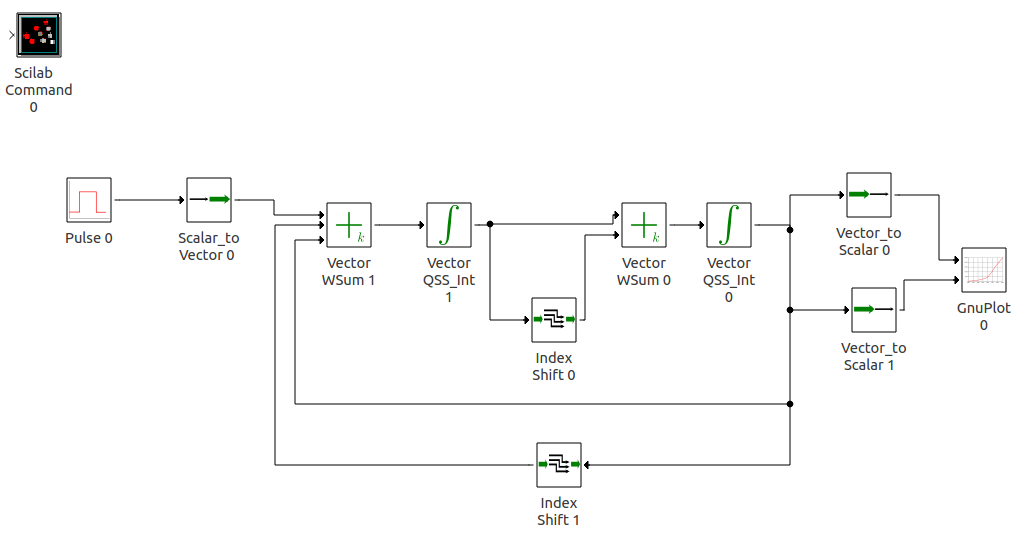
\includegraphics[scale=0.40]{lclines}
  \caption{Modelo PowerDEVS LC Lines }
   \label{fig:lclines}
\end{figure}

\subsection{Control de Energía de un Conjunto de Aires Acondicionados}
Este modelo permite estudiar la dinámica y control del consumo energético de un grupo de equipos de Aire Acondicionados (AA). Consideramos un gran número de equipos de aire acondicionado utilizados para controlar la temperatura de distintas habitaciones. La temperatura en la habitación $i$-ésima $\theta_i(t)$ sigue la ecuación:
%TODO Eliminar el ruido?
\begin{equation*}
\frac{d\theta_i(t)}{dt} = \frac{1}{C_i \cdot R_i } [ \theta_i(t) - \theta_a + R_i \cdot P_i \cdot m_i(t) + w_i(t) ]
\end{equation*}
donde$R_i$ y $C_i$ son parámetros que representan la resistencia y capacitancia térmica de la habitación $i$ respectivamente. $P_i$ es la potencia del equipo de aire acondicionado $i$ cuando se encuentra encendido. $\theta_a$ es la temperatura del ambiente y $w_i(t)$ es un termino de ruido que representa la perturbación térmica.

La variable $m_i (t)$ es el estado del $i$-ésimo equipo de aire acondicionado, que toma como valor $1$ cuando el equipo está encendido ó $0$ en caso contrario. Sigue una ley prendido-apagado de control con histéresis:

\begin{equation}
m_i(t^{+}) = \left\{ 
  \begin{array}{l l}
    0 \text{ si } \theta_i(t) \leq \theta_r(t) - 0.5 \text{ y } m_i(t)=1 \\
    1 \text{ si } \theta_i(t) \geq \theta_r(t) - 0.5 \text{ y } m_i(t)=1 \\
    m_i (t) \text{ caso contrario } 
  \end{array} \right.
\end{equation}

donde $\theta_r(t)$ es la temperatura de referencia calculando por un sistema de control global.
El consumo energético del grupo completo de aires acondicionado se calcula como :

\begin{equation*}
P(t) = \sum_{i=1}^{N}  m_i(t) \cdot P_i
\end{equation*}

Para lograr esto se utiliza una ley de control Proporcional Integral (PI) que calcula la temperatura de referencia como:

\begin{equation*}
\theta_r(t) = K_p \cdot [P_r(t) - P(t)] + K_I \cdot \int_{\tau = 0}^t [P_r(\tau) - P(\tau)] d\tau
\end{equation*}

donde $K_P$ y $K_I$ son parámetros del controlador $PI$.

En este ejemplo utilizamos $N = 2400$ equipos de aires acondicionados y utilizamos los parámetros dados en \cite{PKBW12}, con la excepción del ruido, el cual ignoramos para simplificar la simulación. El modelo resultante es el mostrado en la figura \ref{fig:airs}.

\begin{figure}[!htbp]
  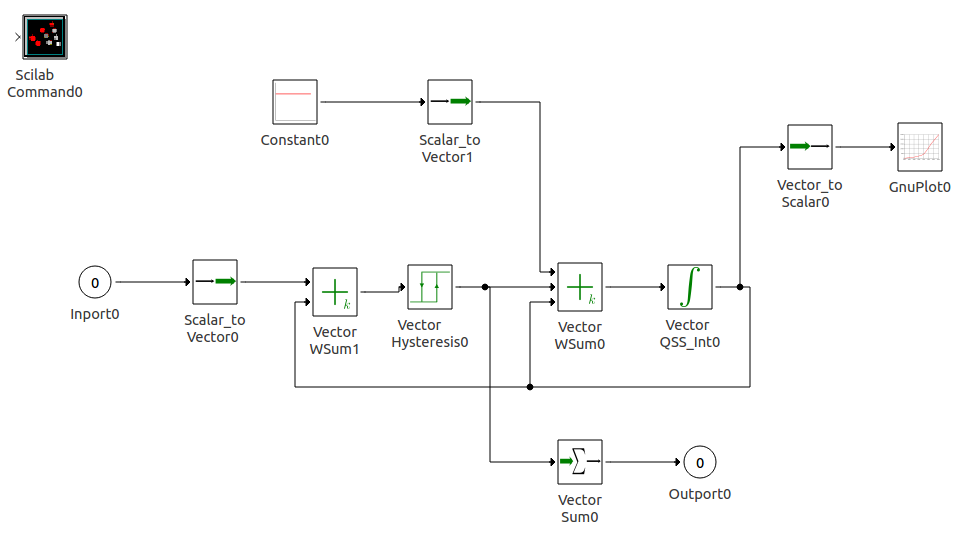
\includegraphics[scale=0.40]{Airs}
  \caption{Modelo PowerDEVS Aires Acondicionado }
   \label{fig:airs}
\end{figure}

\chapter{Detalles de la implementación}
A continuación se presenta el pseudo código que implementa las transformaciones descriptas en este trabajo, el código completo puede encontrarse en \url{https://github.com/lucciano/pd2mo}

El programa esta separado en 4 módulos:
\begin{itemize}
\item Programa principal en el archivo main.cpp, el cual es responsable de la interfaz con el usuario (linea de comando) y lanzar la transformación de la simulación, asi como establecer los archivos desde donde se lee y hacia donde se escriben la simulación de powerDEVS y Modelica, respectivamente.


\begin{function*}[H]
 modelCoupled *cm = parsePDS(QString::fromStdString(src\_infile))\;
 modelCoupled *qm = flatter::flat(cm)\;
 Pd2Mo q = Pd2Mo()\;
 q.transform(flatted, modelname, \&outfile, \&oFlogfile)\;
 AST\_StoredDefinition sd = parseFile(src\_outfile.c\_str(),\&amp;r)\;
 mda *m = new mda()\;
 prodint *  prod = new prodint()\;
 If *i = new If()\;
 
 outfile $<<$ m$->$visitClass( 
 	prod$->$visitClass( 
 		i$->$visitClass( 
 		\*sd$->$models()$->$begin()))) $<<$ endl\;
 \caption{main(src\_infile)}
\end{function*}

\newpage
\item La clase \emph{Pd2Mo} implementa las principales partes de la transformación.

\begin{function}[H]
 modelCoupled *model = parsePDS(qfilename)\;
 AST\_ClassList classList = getAsClassList(model)\; 
 int j = 0\;
 \ForEach{class en classList}{
 	\If{La clase esta traducida a $\mu$Modelica}{
 		Prefijamos las variables con el nombre del modelo $class$ y la posición $j$ que ocupan en la lista\;
 		Remplazamos la entrada $class$ dentro de la lista por su copia producida en el paso anterior\;
 	}
 }
 Creamos un modelo $modeloMo$\;
 \ForEach{class en classList}{ 
 	Combinamos el modelo $class$ con el $modeloMo$\;
 }
 

 \ForEach{ic en Conexión Interna del Modelo}{
	\tcc{Las conexiones ic estan definidas como dos pares de números, cada par señalan número  de modelo y número de puerto, en este caso los puertos deben ser desfasados en uno, pues los puertos en nuestra representación son los sub-indices de $u$ e $y$ para cada modelo, pero el primer elemento de los arreglos en Modelica comienzan}
	\If{Si los modelos de ic son Escalares}{
		Se agrega la ecuación que representa la conexión entre los modelos\;
	}\ElseIf{Si los modelos de ic son Vectoriales}{
		Se agregan $N$ ecuaciones indexadas por $i$ que representa la conexión, vectorial entre los modelos mediante una sentencia For\;
	}\Else{
		No se conoce la conexión;
	}
 }
 \caption{Pd2Mo::transform()}
\end{function}

\item La clase \emph{flatter} implementa el aplanado de los modelos acoplados.

\begin{algorithm}[H]
 \ForEach{ModeloHijo en Lista de Modelos}{
 	\If{Tipo de ModeloHijo es COUPLED}{
 		\ForEach{ModeloHijo2 en Lista de ModeloHijo$->$ModeloHijo}{
 			 	\If{Tipo de ModeloHijo2 es ATOMIC}{
 			 		Copiamos el ModeloHijo2 al ModeloResultado\;
 			 	}\Else{
 			 		Copiamos el aplanado de ModeloHijo2\;
 			 	}
 			 	\ForEach{Conexión del Modelo}{
 			 		\If{Si la conexión involucra un modelo "aun no procesado"}{
 			 			Las conexiones deben ser modificadas teniendo en cuenta los modelos agregados en el aplanado\;
 			 		}
 			 		\If{Si la conexión involucra como destino el modelo acoplado ModeloHijo}{
 			 			Se crea una nueva conexión (en ModeloResultado) entre los modelos agregado recientemente según la conexión del puerto de entrada del ModeloHijo y el origen de la conexión\;
 			 			La conexión se marca para ser borrada\;
 			 		}
 			 		\If{Si la conexión involucra como origen el modelo acoplado ModeloHijo}{
 			 			Se crea una nueva conexión (en ModeloResultado) entre los modelos agregado recientemente según la conexión del puerto de salida del ModeloHijo y el destino de la conexión\;
 			 			La conexión se marca para ser borrada
 			 		}
 			 		\If{Si la conexión fue marcada}{Se borra la conexión}
 			 	}
 		}
 		
 	}\Else{
 		Copiamos el nodo ModeloHijo al ModeloResultado \;
 		Copiamos las conexiones del ModeloHijo y cualquier otro ModeloHijo que ya haya sido procesado
 	}
 }
 return ModeloResultado
 \caption{flatter::flat}
\end{algorithm}

\item La clase \emph{mda}, \emph{prodint}, \emph{If} implementan transformaciones enfocadas en $\mu$Modelica.
\end{itemize}

Tanto la clase $mda$, $prodint$ y $If$ recorren el árbol abstracto sintáctico (AST), por lo que cada clase es implementada heredando de una clase común (Traverser), la cual retorna una copia del AST y remplaza una parte este.

 \begin{itemize}
 	\item  $mda$: Remplaza expresiones de la forma $X[N,k]$, donde $k \in \mathbb{N}$ o evaluá a una variable que evaluá a una expresión $\in \mathbb{N}$, es remplazado por $X_k[N]$
 	
 	\item $prodint$: Remplaza expresiones de la forma $u[i, 1:nin] * w$ por expresiones de la forma u[i,1] * w[1] + u[i,2] * w[2] .... + u[i,nin] * w[nin], donde $nin \in \mathbb{N}$ o evaluá a una variable que evaluá a una expresión $\in \mathbb{N}$
 	
 	\item $If$: Remplaza expresiones de la forma $if(v){eq_1}else{eq_2}$ si $v$ evaluá a un booleano (a partir de parámetros o constantes, es decir en análisis estático) se remplaza por $eq_1$ o $eq_2$ si es $v$ es verdadero o falso respectivamente.
 \end{itemize}


\chapter{Conclusiones y Trabajo a futuro}
En este capitulo mostramos los resultados del presente trabajo, comparamos los resultados de la ejecución de 5 modelos, los tiempos de ejecución y comparamos los resultados obtenidos.

\section{Resultados}

\section{Modelos}
A continuación por cada uno de los modelos se muestra una gráfica de valores en tiempo de las simulaciones, a la izquierda se muestra el resultado en PowerDEVS y a la derecha los de QSS-Solver.

\subsubsection{lcline}
\begin{figure}[H]
\centering
\begin{minipage}{0.5\textwidth}
\centering
 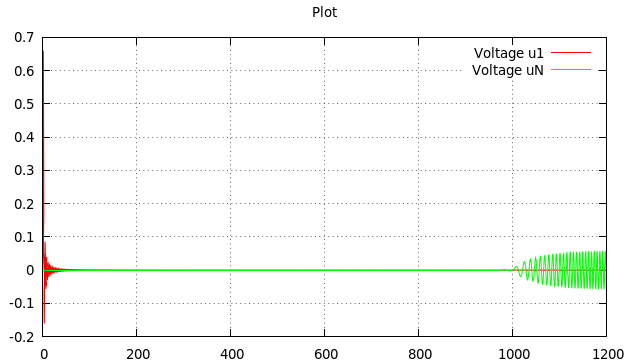
\includegraphics[width=\linewidth]{lcline-pd}
\end{minipage}\hfill
\begin{minipage}{0.5\textwidth}
\centering
 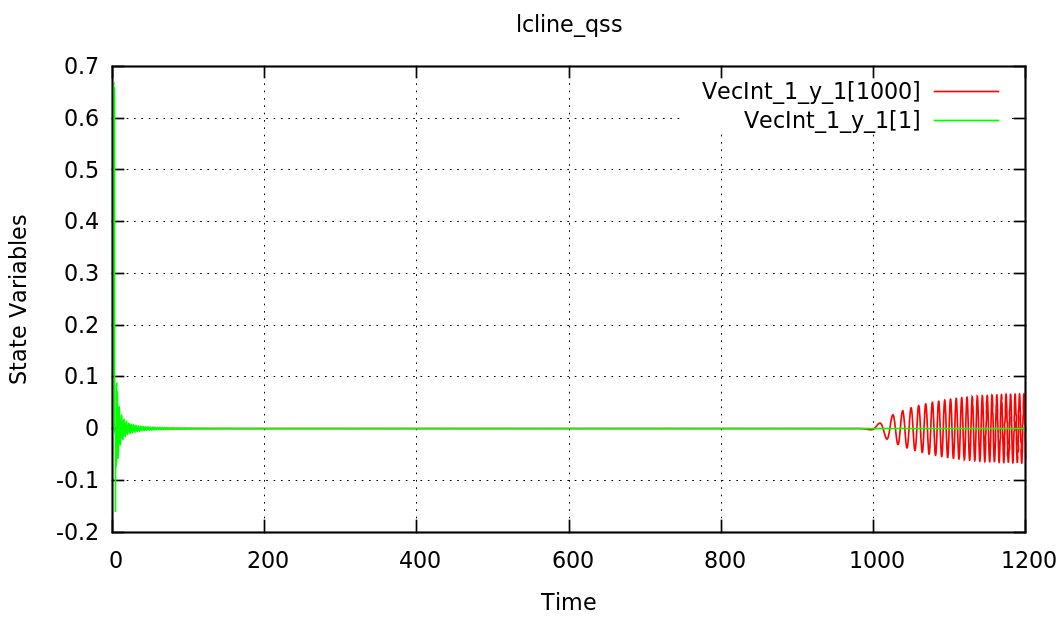
\includegraphics[width=\linewidth]{lcline-qss}
\end{minipage}
\end{figure}

\subsubsection{inversers}

\begin{figure}[H]
\centering
\begin{minipage}{0.5\textwidth}
\centering
 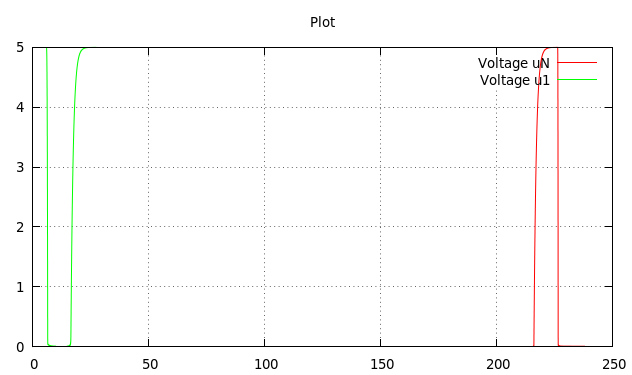
\includegraphics[width=\linewidth]{inversers-pd}
\end{minipage}\hfill
\begin{minipage}{0.5\textwidth}
\centering
 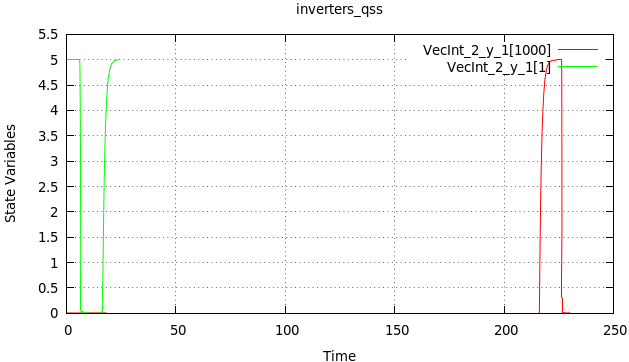
\includegraphics[width=\linewidth]{inversers-qss}
\end{minipage}
\end{figure}

\subsubsection{adr}

\begin{figure}[H]
\centering
\begin{minipage}{0.5\textwidth}
\centering
 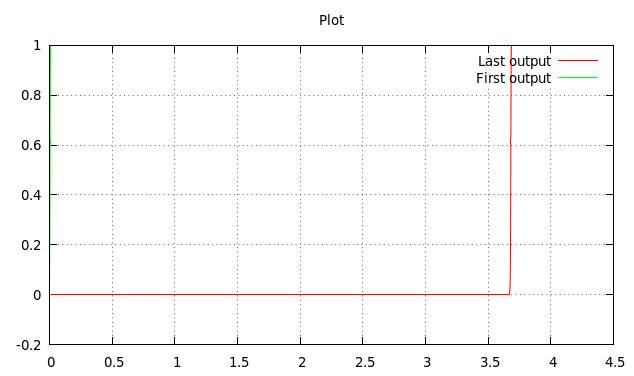
\includegraphics[width=\linewidth]{adr-pd}
\end{minipage}\hfill
\begin{minipage}{0.5\textwidth}
\centering
 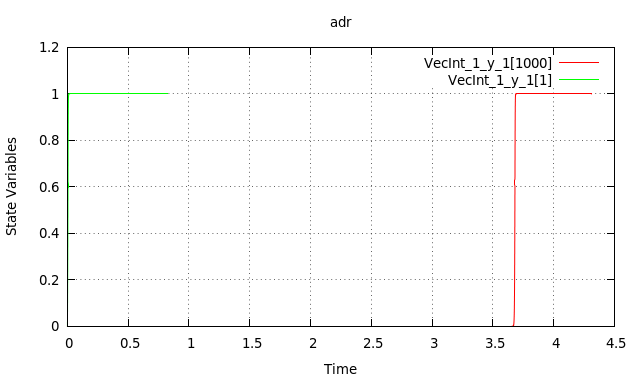
\includegraphics[width=\linewidth]{adr-qss}
\end{minipage}
\end{figure}

\subsubsection{buck\_disk}

\begin{figure}[H]
\centering
\begin{minipage}{0.5\textwidth}
\centering
 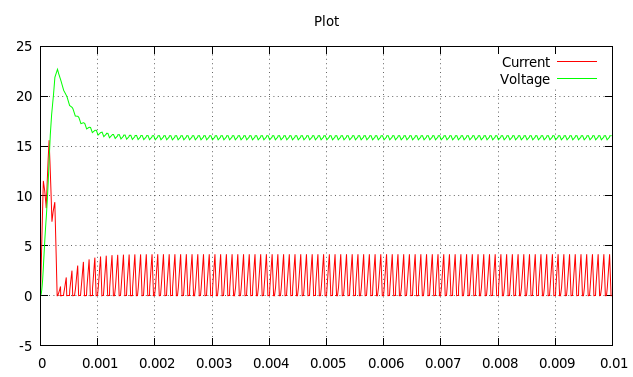
\includegraphics[width=\linewidth]{buck_disk-pd}
\end{minipage}\hfill
\begin{minipage}{0.5\textwidth}
\centering
 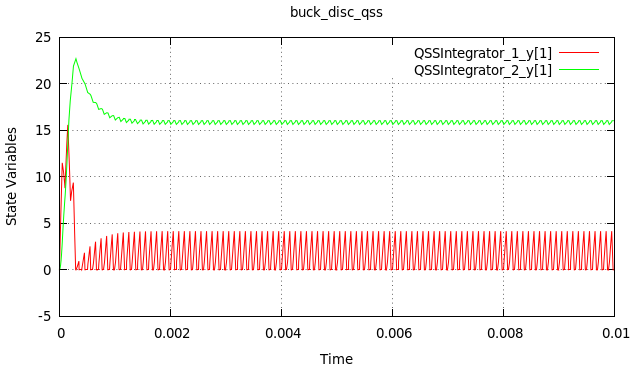
\includegraphics[width=\linewidth]{buck_disk-qss}
\end{minipage}
\end{figure}

\subsubsection{lotka\_voltera}

\begin{figure}[H]
\centering
\begin{minipage}{0.5\textwidth}
\centering
 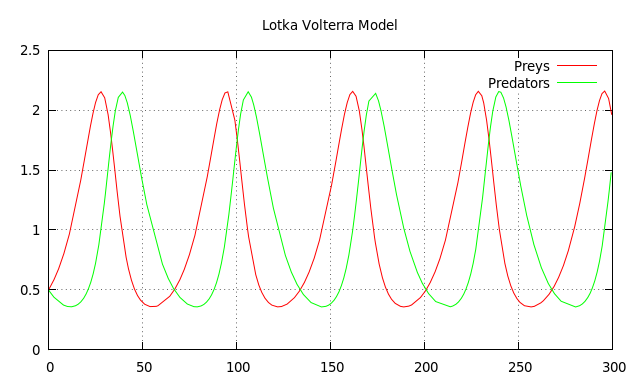
\includegraphics[width=\linewidth]{lotka_voltera-pd}
\end{minipage}\hfill
\begin{minipage}{0.5\textwidth}
\centering
 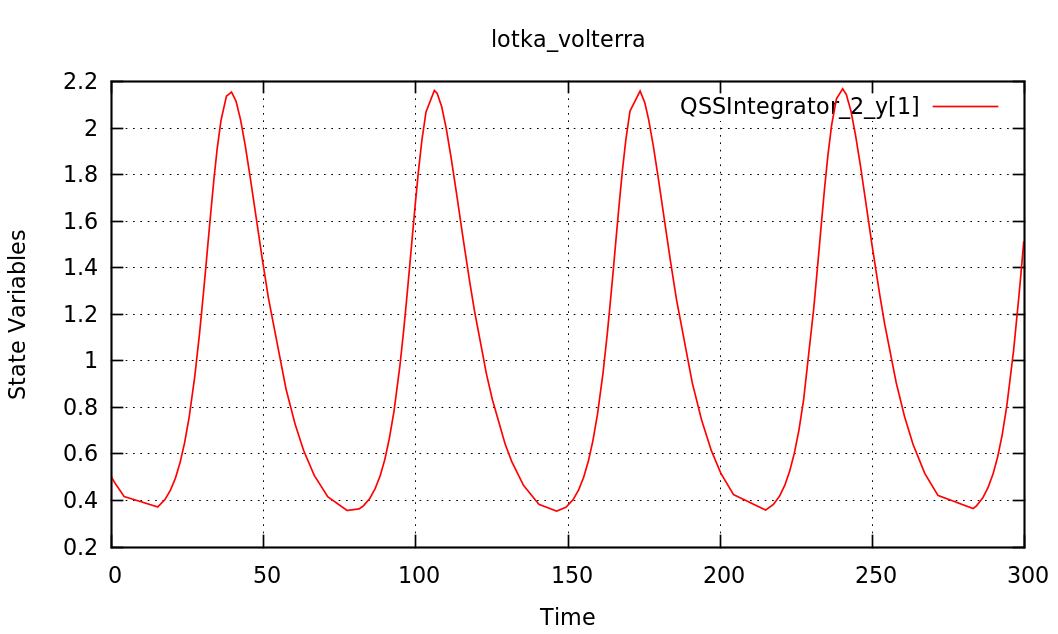
\includegraphics[width=\linewidth]{lotka_voltera-qss}
\end{minipage}
\end{figure}

\subsection{Resultados}
\begin{table}[H]
\centering	
\label{my-label}
\begin{tabular}{llllll}
\toprule
{\bf Modelos}            &  {\bf P.DEVS(ms)} & {\bf QSS-S. (ms)} & {\bf Mejora (\%)} \\
\toprule
lcline 1200s, N=1000     & 40994         & 18458.9         & 45          \\
inversers 250s, N=1000   & 4749          & 1897.22         & 39.9        \\
adr (LIQSS2) 10s, N=1000 & 7467          & 1412.06         & 18.9        \\
buck\_disk  0.1s,        & 343           & 15.2497         & 4.4         \\
lotka\_voltera 300s      & 52            & 0.476385        & 0.91
\end{tabular}
\end{table}

\nocite{*}

\bibliographystyle{plain}
\bibliography{tesina_luciano}

\end{document}
